\documentclass[11pt]{article}

\usepackage{graphicx}
\usepackage{csquotes}
\usepackage{courier}
\setcounter{secnumdepth}{4}

\title{The Point-Plane Problem}
\author{Adam Yedidia}

\begin{document}

\maketitle
    
This is a short essay about a problem in photonics that I call the ``Point-Plane Problem.'' I discuss it because it is a simpler version of the problem that I discussed in Section 2 of \emph{Locating a Target in Three Dimensions}, which concerns finding a forward model in a situation where a divergent source and an unfocussed detector are separated by a Lambertian reflecting wall. \\

This problem, instead, is about finding a forward model for the situation in which a divergent source is firing light in all directions, and some distance away there is a detecting wall (meaning that the entire wall is a detector). As a function of time and of the distance between the source and the wall, we'd like to know how much light is hitting the wall. \\

Fig.~\ref{fig:expandingsphere} is a sketch of what the problem looks like. Our light source is emitting a pulse of light. As time passes, the light is moving through space in an expanding sphere. \\

\begin{figure}
\begin{center}
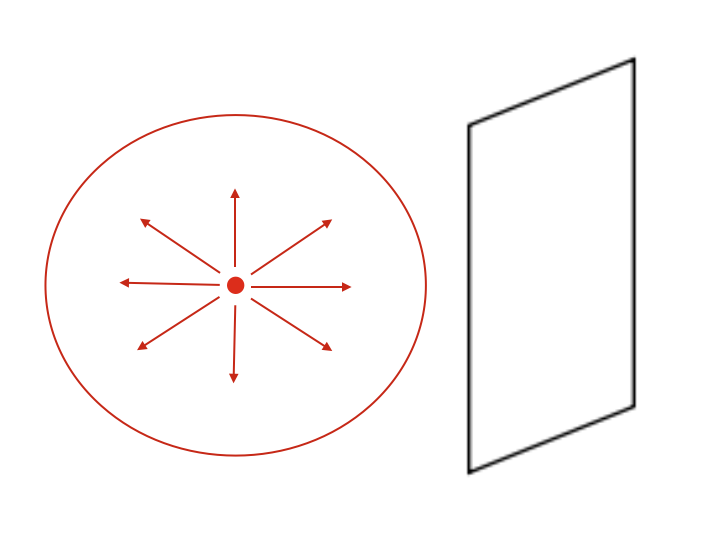
\includegraphics[scale=0.6]{figs/wallcircle.png} % yeah yeah I know
\caption{The light source is emitting light in all directions, and the light forms a hollow sphere that expands with time. \label{fig:expandingsphere}}
\end{center}
\end{figure}

Fig.~\ref{fig:wallcircle} is a sketch of the situation after enough time has passed for the first light to hit the wall. The light is forming a circle on the wall, which expands as time passes. We'll call the distance from the source to the wall, or alternatively the time of first light, $T$, the amount of time that's passed since first light $t$, and the radius of the circle on the wall $r$.

\begin{figure}
\begin{center}
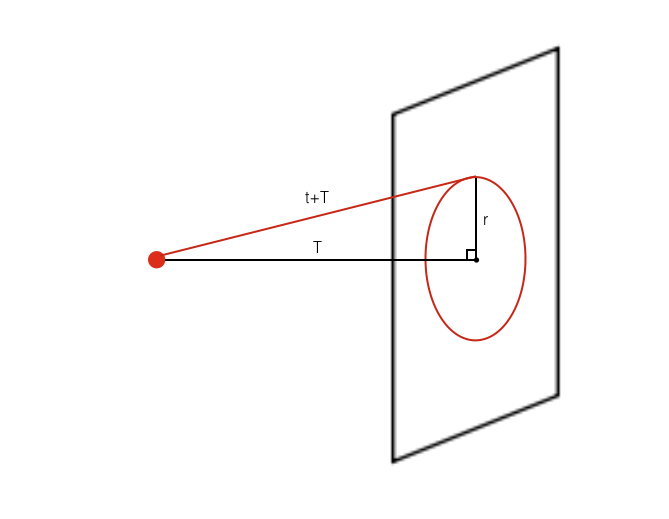
\includegraphics[scale=0.6]{figs/expandingsource.png}
\caption{After first light, the pattern of light on the wall is the cross-section of the expanding sphere---in other words, a circle. \label{fig:wallcircle}}
\end{center}
\end{figure}

\section{Overview}

Now, how can we describe the intensity as a function of time, $I(t)$? Well, we can split into two terms:

$$I(t) = N_p(t) \cdot I_p(t)$$

where $N_p(t)$ describes the number of ``paths'' from the source to the wall---in other words, the number of individual points on the wall that the light hits. In order to do this, we'll want to say that a point on a wall is a little patch on the wall of size $\Delta x \times \Delta x$. $I_p(t)$ describes the intensity per path---for each point hit by a beam, how much intensity is contributed? This will give us the total intensity function exactly, assuming $\Delta x$ is small.

We'll also discretize time into little chunks of size $\Delta t$. This will come in handy later.

\section{Computing $N_p(t)$}

Now, how are we going to go about computing $N_p(t)$? Well, we'll start by computing the number of beams of light that hit the wall since first light $N_c(t)$, because that's easier. That's just the area of the circle divided by the area of a point on the wall.

$$N_c(t) = \frac{\pi r^2}{(\Delta x)^2}$$

Or equivalently (by the Pythagorean theorem),

$$N_c(t) = \frac{\pi((T+t)^2 - T^2)}{(\Delta x)^2}$$

$$N_c(t) = \frac{\pi((2Tt + t^2)}{(\Delta x)^2}$$

Now, because $N_c(t)$ is the cumulative number of paths since first light, we can get the number of paths at any given point in time by taking its derivative.

$$N_p(t) = dN_c(t) = \frac{2\pi(T+t)\Delta t}{(\Delta x)^2}$$

\section{Computing $I_p(t)$}

Next, we need to compute the contribution of each beam of light hitting the wall to the total intensity received by the wall. Naturally, as time passes, we should expect this to decrease, both since the light must travel further before it hits the wall, and because the light is hitting the wall at more of a glancing angle. 

To figure out what fraction of the light hits a given $\Delta x \times \Delta x$ patch on the wall, we'll want to calculate what fraction of the expanding sphere of light is hitting that patch. At time $t$ after first light, the sphere's area will be $4\pi(T+t)^2$, and the area of the patch will be $(Delta x)^2$. Of course, that's not the whole story, because the patch is slanted at an angle of $cos \theta$ from direction of the beam (where $\theta$ is the angle from the beam to the wall's normal vector)---in this case, $\cos \theta$ is easily found to be $\frac{T}{T+t}$.

Thus, the fraction of the expanding sphere that hits the little patch is:

$$I_p(t) = \frac{T}{T+t} \frac{(\Delta x)^2}{4\pi(T+t)^2}$$
$$I_p(t) = \frac{T(\Delta x)^2}{4\pi(T+t)^3}$$

\section{Computing $I(t)$}

Now that we have $N_p(t)$ and $I_p(t)$, we can compute $I(t)$!

$$I(t) = N_p(t) \cdot I_p(t)$$
$$I(t) = \frac{2\pi(T+t)\Delta t}{(\Delta x)^2} \frac{T(\Delta x)^2}{4\pi(T+t)^3}$$
$$I(t) = \frac{T \Delta t}{2 (T+t)^2}$$

In Fig.~\ref{fig:spherepoint} we have a comparison of this theoretical model with the result of a simulation. The simulation is run by discretizing the wall into many little points, and for each point adding the amount of light calculated to have arrived at that point into the appropriate bin in a time histogram. (For a more detailed explanation of the simulation process, see Section 3 of \emph{Locating a Target in Three Dimensions}.) As we can see, the theory perfectly matches simulation, except at the very end when we taper off because the simulated wall is finite in size.

\begin{figure}
\begin{center}
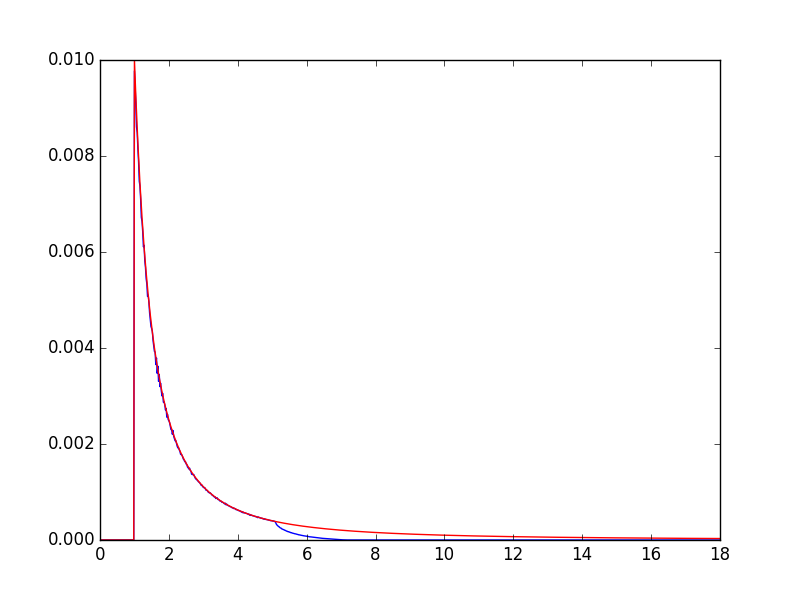
\includegraphics[scale=0.6]{figs/spherepoint.png}
\caption{This is a graph of the fraction of emitted light that hits the wall ($y$-axis) as a function of time ($x$-axis). The theory is in red and the simulation is in blue. \label{fig:spherepoint}}
\end{center}
\end{figure}

It is somewhat unintuitive that there is a sudden jump from 0 light to the peak amount of light at first light. The best intuition I can give for this beyond just the math is that the radius of the circle on the wall, $r$, given by $\sqrt{(T+t)^2 - T^2}$---so at $t \approx T$, $\frac{dr}{dt}$ is going to be huge! So we should not be shocked to see discontinuities here.

\end{document}